% --- chapter
\newcommand{\chapter}[2][]{
	\newcommand{\chapname}{#2}
	\begin{flushleft}
		\begin{minipage}[t]{\linewidth}
			
\includegraphics[height=1cm]{hdht-logo.png}
			\hspace{0pt}	
			\sffamily\bfseries\large Bài  26. Các loại quang phổ
			\begin{flushleft}
				\huge\bfseries #1
			\end{flushleft}
		\end{minipage}
	\end{flushleft}
	\vspace{1cm}
	\normalfont\normalsize
}
%-----------------------------------------------------
\chapter[Máy quang phổ]{Máy quang phổ}


Máy quang phổ là dụng cụ để phân tích một chùm ánh sáng phức tạp thành những thành phần đơn sắc.
\subsection{Cấu tạo}
Máy quang phổ lăng kính gồm 3 bộ phận chính: ống chuẩn trực, hệ tán sắc và buồng ảnh.
\begin{description}
	\item[Ống chuẩn trực] gồm hệ thấu kính đặt đồng trục, có tác dụng làm chùm sáng từ vật cần đo qua ống cho chùm tia ló song song.
	\item[Hệ tán sắc] gồm một lăng kính (hoặc hệ lăng kính), có tác dụng phân tách chùm sáng song song khi qua ống chuẩn trực thành nhiều chùm tia đơn sắc, song song.
	\item[Buồng tối (buồng ảnh)] là một hộp kín có chứa kính ảnh đặt tại tiêu diện ảnh của thấu kính hội tụ, có tác dụng quan sát quang phổ.
\end{description} 	
	\begin{center}
		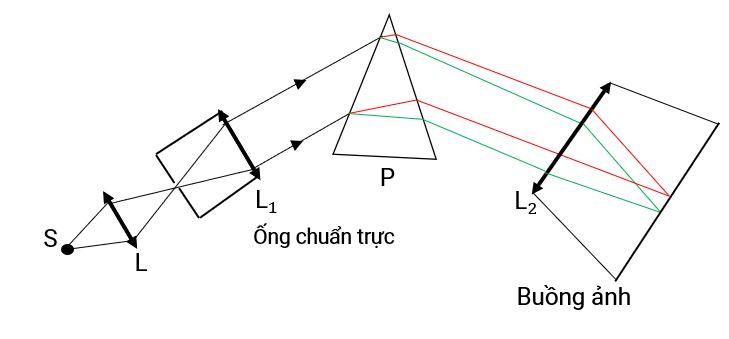
\includegraphics[scale=1]{../figs/VN12-PH-36-L-021-1-1.JPG}
	\end{center}
	\subsection{Nguyên tắc hoạt động}
Nguyên tắc hoạt động của máy quang phổ lăng kính dựa trên hiện tượng tán sắc ánh sáng.
\begin{itemize}

\item Sau khi ló ra khỏi ống chuẩn trực, chùm ánh sáng sẽ trở thành một chùm song song. 

\item Chùm này qua lăng kính sẽ bị phân tách thành nhiều chùm đơn sắc song song, lệch theo các phương khác nhau. 

\item Mỗi chùm sáng đơn sắc được thấu kính hội tụ thành một vạch trên tiêu diện, đó là một vạch màu. 

\item Các vạch màu này được chụp trên kính ảnh hoặc hiện lên tấm kính mờ. Mỗi vạch màu ứng với một bước sóng xác định, gọi là vạch quang phổ. 
\item Tập hợp các vạch quang phổ chụp được làm thành quang phổ của nguồn.

\end{itemize}
